% begin module areas-ex1
\begin{frame}
\begin{example}
Find the sum of the areas of the four approximating rectangles obtained using right endpoints.
\begin{columns}[c]
\column{.5\textwidth}
\begin{itemize}
\item<2->  Let $R_4$ denote the sum of the areas of the rectangles.
\item<3-| alert@3-4>  Each rectangle has width $\fcAnswer{4}{\frac{1}{4}}$.
\item<5-| alert@5-6>  The heights are $\fcAnswer{6}{\left( \frac{1}{4}\right)^2}, \fcAnswer{6}{\left( \frac{1}{2}\right)^2}, \fcAnswer{6}{\left(\frac{3}{4}\right)^2}$, and $\fcAnswer{6}{1^2}$.
\item<handout:2-| 9->  A similar calculation works for $L_4$, the sum of the areas of the left endpoint rectangles.
\end{itemize}
\column{.5\textwidth}
\psset{xunit=3cm, yunit=3cm}
\begin{pspicture}(-0.3, -0.3)(1.2,1.2)
\psframe*[linecolor=white](-5,-5)(5,5)
\psaxes[ticks=none, labels=none]{<->}(0,0)(-0.3,-0.3)(1.2,1.2)
\tiny
\only<handout:1|-8>{
\psline*[linecolor=\fcColorAreaUnderGraph, linewidth=0.1pt](0.25, 0)(0.25, 0.0625)(0, 0.0625)(0, 0)(0.5, 0)(0.5, 0.25)(0.25, 0.25)(0.25, 0)(0.75, 0)(0.75, 0.5625)(0.5, 0.5625)(0.5, 0)(1, 0)(1, 1)(0.75, 1)(0.75, 0)
\psline[linecolor=blue, linewidth=0.1pt](0.25, 0)(0.25, 0.0625)(0, 0.0625)(0, 0)(0.5, 0)(0.5, 0.25)(0.25, 0.25)(0.25, 0)(0.75, 0)(0.75, 0.5625)(0.5, 0.5625)(0.5, 0)(1, 0)(1, 1)(0.75, 1)(0.75, 0)
}
\only<handout:0|10>{
\psline*[linecolor=gray!35, linewidth=0.1pt](0.25, 0)(0.25, 0.0625)(0, 0.0625)(0, 0)(0.5, 0)(0.5, 0.25)(0.25, 0.25)(0.25, 0)(0.75, 0)(0.75, 0.5625)(0.5, 0.5625)(0.5, 0)
%\psline*[linecolor=gray!10](1, 0)(1, 1)(0.75, 1)(0.75, 0)
\psline[linecolor=blue, linewidth=0.1pt](0.25, 0)(0.25, 0.0625)(0, 0.0625)(0, 0)(0.5, 0)(0.5, 0.25)(0.25, 0.25)(0.25, 0)(0.75, 0)(0.75, 0.5625)(0.5, 0.5625)(0.5, 0)(1, 0)(1, 1)(0.75, 1)(0.75, 0)
}
\only<handout:2|9->{
\psline*[linecolor=\fcColorAreaUnderGraph, linewidth=0.1pt](0, 0)(0, 0)(0.25, 0)(0.25, 0)(0.25, 0)(0.25, 0.0625)(0.5, 0.0625)(0.5, 0)(0.5, 0)(0.5, 0.25)(0.75, 0.25)(0.75, 0)(0.75, 0)(0.75, 0.5625)(1, 0.5625)(1, 0)
\psline[linecolor=blue, linewidth=0.1pt](0, 0)(0, 0)(0.25, 0)(0.25, 0)(0.25, 0)(0.25, 0.0625)(0.5, 0.0625)(0.5, 0)(0.5, 0)(0.5, 0.25)(0.75, 0.25)(0.75, 0)(0.75, 0)(0.75, 0.5625)(1, 0.5625)(1, 0)
}
\rput[t](0.25,-0.03){$\frac{1}{4}$}\rput[t](0.5,-0.03){$\frac{1}{2}$}\rput[t](0.75,-0.03){$\frac{3}{4}$}\rput[t](1,-0.03){$1$}
%Function formula: (x)^{2}
\rput[t](0.5,1){$y=x^{2}$}
\psplot[linecolor=red, plotpoints=1000]{0}{1}{x 2 exp }
\end{pspicture}
%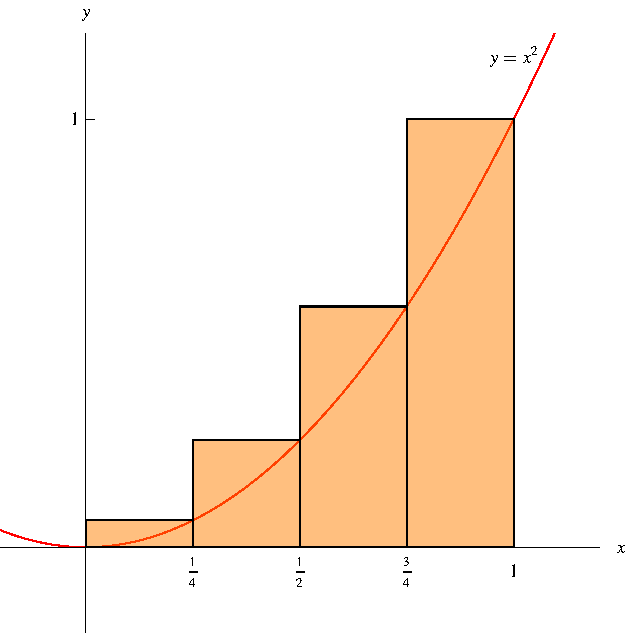
\includegraphics[height=4.5cm]{integration/pictures/05-01-rightb.pdf}%
\end{columns}
\uncover<7->{%
\abovedisplayskip=0pt
\belowdisplayskip=0pt
\[
R_4 = \alertNoH{10}{\frac{1}{4}\cdot \left(\frac{1}{4}\right)^2}%
+ \alertNoH{10}{\frac{1}{4}\cdot \left(\frac{1}{2}\right)^2}%
+ \alertNoH{10}{\frac{1}{4}\cdot \left(\frac{3}{4}\right)^2}%
+ \frac{1}{4}\cdot \left( 1\right)^2%
\uncover<8->{ = \frac{15}{32} = 0.46875}%
\]
}%
\uncover<handout:2-| 9,10,11->{%
\abovedisplayskip=0pt
\belowdisplayskip=0pt
\[
L_4 = \frac{1}{4}\cdot \left( 0\right)^2%
+\alertNoH{10}{ \frac{1}{4}\cdot \left(\frac{1}{4}\right)^2}%
+ \alertNoH{10}{\frac{1}{4}\cdot \left(\frac{1}{2}\right)^2}%
+\alertNoH{10}{ \frac{1}{4}\cdot \left( \frac{3}{4}\right)^2}%
\uncover<11->{ = \frac{7}{32} = 0.21875}%
\]
}%
\vspace{-.1in}
\end{example}
\end{frame}
% end module areas-ex1
